\section{Introduction}
\label{sec:introduction}

Multi-agent AI systems increasingly rely on \emph{trust dynamics}: each agent
maintains a weight vector or matrix encoding its confidence in peer agents'
specialized capabilities.  As the swarm executes tasks, these weights are updated and
propagated through aggregation operators — most commonly Sinkhorn--Knopp normalization,
which projects the raw trust matrix onto the Birkhoff polytope of doubly stochastic
matrices \cite{sinkhorn1964relationship,sinkhorn1967concerning}.

The Birkhoff polytope is mathematically attractive.  Its vertices are permutation
matrices, representing maximally specialized routing; its centroid is the uniform
matrix $J/n$ (where $J$ is the all-ones matrix), representing maximal entropy.
Sinkhorn--Knopp converges to this set from any positive matrix.  What is less
appreciated is the \emph{long-run behavior} under repeated application: iterated
Sinkhorn normalization drives trust matrices toward $J/n$, erasing all heterogeneity.

\paragraph{The collapse phenomenon.}
We term this failure mode \textbf{Birkhoff Uniformity Collapse} (BUC).  Figure
\ref{fig:birkhoff_collapse} illustrates the dynamics: for $n{=}50$ agents, variance
retention (the fraction of initial eigenvalue variance that survives to cycle $k$) falls
monotonically from $100\%$ at initialization to $0\%$ at cycle $10$, and remains at
$0\%$ thereafter.  At $n{=}10$, collapse is faster: $0\%$ by cycle $6$.  Collapse is
\emph{not} a numerical artifact; it is a direct consequence of the spectral gap of the
doubly stochastic semigroup — the second eigenvalue of a doubly stochastic matrix
satisfies $|\lambda_2| \leq 1$, and repeated composition drives the matrix toward the
rank-1 steady state proportional to $\mathbf{1}\mathbf{1}^\top/n$.

BUC is catastrophic for specialization-dependent multi-agent systems.  A swarm where
all agents are trusted equally for all tasks cannot route work to the right specialist.
Constitutional governance systems that rely on diversity of agent perspective
\cite{bai2022constitutional} are particularly vulnerable: if trust collapse makes all
agents interchangeable, the MACI separation of Proposer/Validator/Executor breaks down
structurally.

\begin{figure}[t]
  \centering
  % TikZ/PGFPlots figure: Birkhoff Uniformity Collapse
% Usage: % TikZ/PGFPlots figure: Birkhoff Uniformity Collapse
% Usage: % TikZ/PGFPlots figure: Birkhoff Uniformity Collapse
% Usage: \input{figures/birkhoff_collapse} inside a figure environment
%
% Shows variance retention (%) vs cycle k for:
%   - Sinkhorn n=50 (collapses to 0% by cycle 10)
%   - Sinkhorn n=10 (collapses to 0% by cycle 6)
%   - SpectralSphere+residual n=50 (stable at 142%)
%   - SpectralSphere+residual n=10 (stable at 20%)

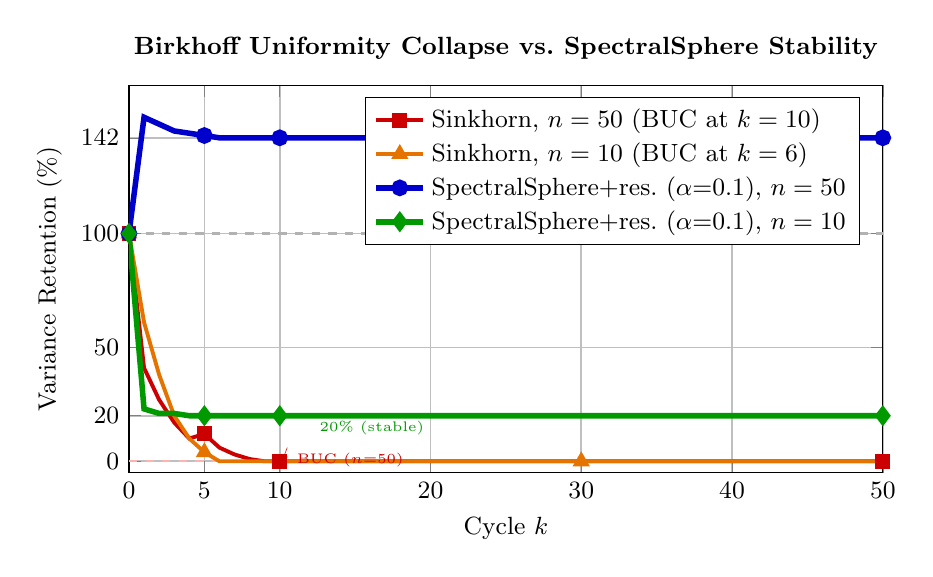
\begin{tikzpicture}
  \begin{axis}[
    width=0.92\linewidth,
    height=6.5cm,
    xlabel={Cycle $k$},
    ylabel={Variance Retention (\%)},
    xmin=0, xmax=50,
    ymin=-5, ymax=165,
    xtick={0,5,10,20,30,40,50},
    ytick={0,20,50,100,142},
    yticklabels={0, 20, 50, 100, 142},
    grid=both,
    grid style={line width=0.3pt, draw=gray!30},
    major grid style={line width=0.6pt, draw=gray!50},
    legend pos=north east,
    legend style={font=\small, cells={anchor=west}},
    tick label style={font=\small},
    label style={font=\small},
    title style={font=\small\bfseries},
    title={Birkhoff Uniformity Collapse vs.\ SpectralSphere Stability},
    clip=true,
  ]

  %% Reference lines
  \draw[dashed, gray!60, line width=0.8pt] (axis cs:0,100) -- (axis cs:50,100)
    node[right, font=\tiny, gray] {100\%};
  \draw[dashed, red!30, line width=0.8pt] (axis cs:0,0) -- (axis cs:50,0);

  %% Sinkhorn n=50: collapses by cycle 10
  \addplot[
    color=red!80!black,
    line width=1.4pt,
    mark=square*,
    mark size=2.0pt,
    mark repeat=5,
  ] coordinates {
    (0,100) (1,41) (2,27) (3,17) (4,10) (5,12) (6,6) (7,3) (8,1) (9,0)
    (10,0) (15,0) (20,0) (30,0) (40,0) (50,0)
  };
  \addlegendentry{Sinkhorn, $n=50$ (BUC at $k=10$)}

  %% Sinkhorn n=10: collapses faster, by cycle 6
  \addplot[
    color=orange!90!black,
    line width=1.4pt,
    mark=triangle*,
    mark size=2.2pt,
    mark repeat=5,
  ] coordinates {
    (0,100) (1,61) (2,38) (3,20) (4,10) (5,4) (6,0)
    (10,0) (15,0) (20,0) (30,0) (40,0) (50,0)
  };
  \addlegendentry{Sinkhorn, $n=10$ (BUC at $k=6$)}

  %% SpectralSphere + residual n=50: stable at 142%
  \addplot[
    color=blue!80!black,
    line width=2.0pt,
    mark=*,
    mark size=2.0pt,
    mark repeat=5,
  ] coordinates {
    (0,100) (1,151) (2,148) (3,145) (4,144) (5,143) (6,142) (7,142)
    (8,142) (9,142) (10,142) (15,142) (20,142) (30,142) (40,142) (50,142)
  };
  \addlegendentry{SpectralSphere+res.\ ($\alpha{=}0.1$), $n=50$}

  %% SpectralSphere + residual n=10: stable at 20%
  \addplot[
    color=green!60!black,
    line width=2.0pt,
    mark=diamond*,
    mark size=2.2pt,
    mark repeat=5,
  ] coordinates {
    (0,100) (1,23) (2,21) (3,21) (4,20) (5,20) (6,20) (7,20)
    (8,20) (9,20) (10,20) (15,20) (20,20) (30,20) (40,20) (50,20)
  };
  \addlegendentry{SpectralSphere+res.\ ($\alpha{=}0.1$), $n=10$}

  %% Annotation: collapse point n=50
  \node[font=\tiny, red!80!black, anchor=north west] at (axis cs:10.5,8)
    {BUC ($n{=}50$)};
  \draw[->, red!80!black, very thin] (axis cs:10.5,6) -- (axis cs:10.2,1);

  %% Annotation: stable equilibrium n=50
  \node[font=\tiny, blue!80!black, anchor=south west] at (axis cs:20,143)
    {$142\%$ (stable)};

  %% Annotation: stable equilibrium n=10
  \node[font=\tiny, green!60!black, anchor=north west] at (axis cs:12,22)
    {$20\%$ (stable)};

  \end{axis}
\end{tikzpicture}
 inside a figure environment
%
% Shows variance retention (%) vs cycle k for:
%   - Sinkhorn n=50 (collapses to 0% by cycle 10)
%   - Sinkhorn n=10 (collapses to 0% by cycle 6)
%   - SpectralSphere+residual n=50 (stable at 142%)
%   - SpectralSphere+residual n=10 (stable at 20%)

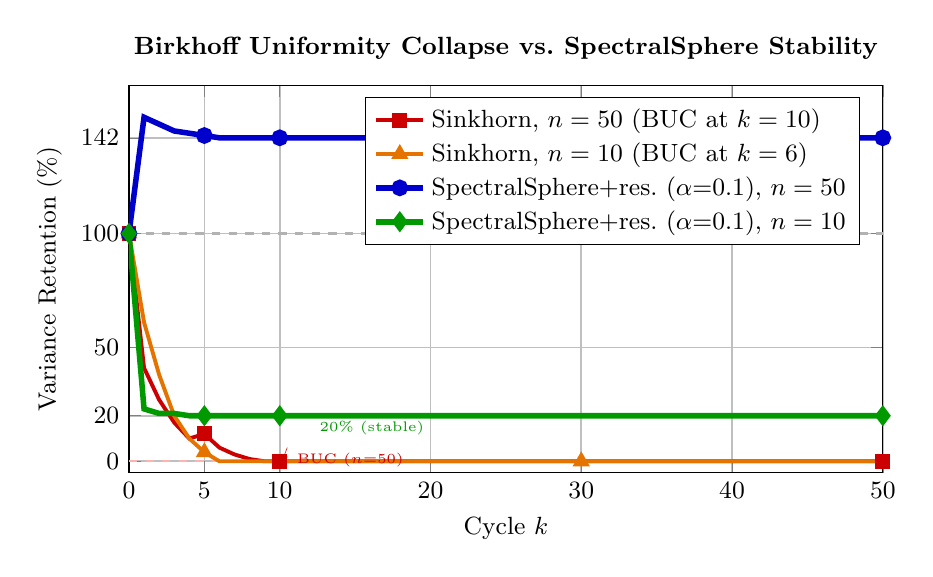
\begin{tikzpicture}
  \begin{axis}[
    width=0.92\linewidth,
    height=6.5cm,
    xlabel={Cycle $k$},
    ylabel={Variance Retention (\%)},
    xmin=0, xmax=50,
    ymin=-5, ymax=165,
    xtick={0,5,10,20,30,40,50},
    ytick={0,20,50,100,142},
    yticklabels={0, 20, 50, 100, 142},
    grid=both,
    grid style={line width=0.3pt, draw=gray!30},
    major grid style={line width=0.6pt, draw=gray!50},
    legend pos=north east,
    legend style={font=\small, cells={anchor=west}},
    tick label style={font=\small},
    label style={font=\small},
    title style={font=\small\bfseries},
    title={Birkhoff Uniformity Collapse vs.\ SpectralSphere Stability},
    clip=true,
  ]

  %% Reference lines
  \draw[dashed, gray!60, line width=0.8pt] (axis cs:0,100) -- (axis cs:50,100)
    node[right, font=\tiny, gray] {100\%};
  \draw[dashed, red!30, line width=0.8pt] (axis cs:0,0) -- (axis cs:50,0);

  %% Sinkhorn n=50: collapses by cycle 10
  \addplot[
    color=red!80!black,
    line width=1.4pt,
    mark=square*,
    mark size=2.0pt,
    mark repeat=5,
  ] coordinates {
    (0,100) (1,41) (2,27) (3,17) (4,10) (5,12) (6,6) (7,3) (8,1) (9,0)
    (10,0) (15,0) (20,0) (30,0) (40,0) (50,0)
  };
  \addlegendentry{Sinkhorn, $n=50$ (BUC at $k=10$)}

  %% Sinkhorn n=10: collapses faster, by cycle 6
  \addplot[
    color=orange!90!black,
    line width=1.4pt,
    mark=triangle*,
    mark size=2.2pt,
    mark repeat=5,
  ] coordinates {
    (0,100) (1,61) (2,38) (3,20) (4,10) (5,4) (6,0)
    (10,0) (15,0) (20,0) (30,0) (40,0) (50,0)
  };
  \addlegendentry{Sinkhorn, $n=10$ (BUC at $k=6$)}

  %% SpectralSphere + residual n=50: stable at 142%
  \addplot[
    color=blue!80!black,
    line width=2.0pt,
    mark=*,
    mark size=2.0pt,
    mark repeat=5,
  ] coordinates {
    (0,100) (1,151) (2,148) (3,145) (4,144) (5,143) (6,142) (7,142)
    (8,142) (9,142) (10,142) (15,142) (20,142) (30,142) (40,142) (50,142)
  };
  \addlegendentry{SpectralSphere+res.\ ($\alpha{=}0.1$), $n=50$}

  %% SpectralSphere + residual n=10: stable at 20%
  \addplot[
    color=green!60!black,
    line width=2.0pt,
    mark=diamond*,
    mark size=2.2pt,
    mark repeat=5,
  ] coordinates {
    (0,100) (1,23) (2,21) (3,21) (4,20) (5,20) (6,20) (7,20)
    (8,20) (9,20) (10,20) (15,20) (20,20) (30,20) (40,20) (50,20)
  };
  \addlegendentry{SpectralSphere+res.\ ($\alpha{=}0.1$), $n=10$}

  %% Annotation: collapse point n=50
  \node[font=\tiny, red!80!black, anchor=north west] at (axis cs:10.5,8)
    {BUC ($n{=}50$)};
  \draw[->, red!80!black, very thin] (axis cs:10.5,6) -- (axis cs:10.2,1);

  %% Annotation: stable equilibrium n=50
  \node[font=\tiny, blue!80!black, anchor=south west] at (axis cs:20,143)
    {$142\%$ (stable)};

  %% Annotation: stable equilibrium n=10
  \node[font=\tiny, green!60!black, anchor=north west] at (axis cs:12,22)
    {$20\%$ (stable)};

  \end{axis}
\end{tikzpicture}
 inside a figure environment
%
% Shows variance retention (%) vs cycle k for:
%   - Sinkhorn n=50 (collapses to 0% by cycle 10)
%   - Sinkhorn n=10 (collapses to 0% by cycle 6)
%   - SpectralSphere+residual n=50 (stable at 142%)
%   - SpectralSphere+residual n=10 (stable at 20%)

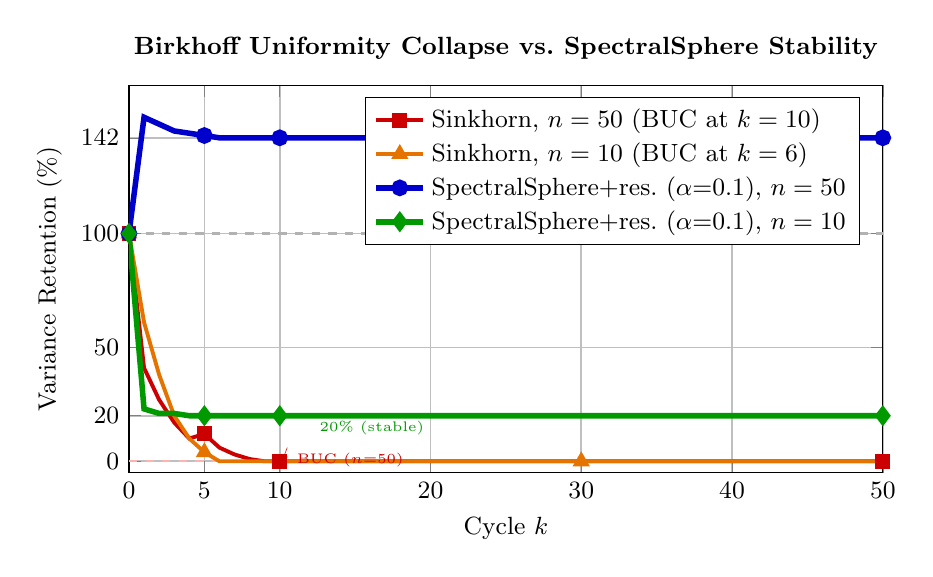
\begin{tikzpicture}
  \begin{axis}[
    width=0.92\linewidth,
    height=6.5cm,
    xlabel={Cycle $k$},
    ylabel={Variance Retention (\%)},
    xmin=0, xmax=50,
    ymin=-5, ymax=165,
    xtick={0,5,10,20,30,40,50},
    ytick={0,20,50,100,142},
    yticklabels={0, 20, 50, 100, 142},
    grid=both,
    grid style={line width=0.3pt, draw=gray!30},
    major grid style={line width=0.6pt, draw=gray!50},
    legend pos=north east,
    legend style={font=\small, cells={anchor=west}},
    tick label style={font=\small},
    label style={font=\small},
    title style={font=\small\bfseries},
    title={Birkhoff Uniformity Collapse vs.\ SpectralSphere Stability},
    clip=true,
  ]

  %% Reference lines
  \draw[dashed, gray!60, line width=0.8pt] (axis cs:0,100) -- (axis cs:50,100)
    node[right, font=\tiny, gray] {100\%};
  \draw[dashed, red!30, line width=0.8pt] (axis cs:0,0) -- (axis cs:50,0);

  %% Sinkhorn n=50: collapses by cycle 10
  \addplot[
    color=red!80!black,
    line width=1.4pt,
    mark=square*,
    mark size=2.0pt,
    mark repeat=5,
  ] coordinates {
    (0,100) (1,41) (2,27) (3,17) (4,10) (5,12) (6,6) (7,3) (8,1) (9,0)
    (10,0) (15,0) (20,0) (30,0) (40,0) (50,0)
  };
  \addlegendentry{Sinkhorn, $n=50$ (BUC at $k=10$)}

  %% Sinkhorn n=10: collapses faster, by cycle 6
  \addplot[
    color=orange!90!black,
    line width=1.4pt,
    mark=triangle*,
    mark size=2.2pt,
    mark repeat=5,
  ] coordinates {
    (0,100) (1,61) (2,38) (3,20) (4,10) (5,4) (6,0)
    (10,0) (15,0) (20,0) (30,0) (40,0) (50,0)
  };
  \addlegendentry{Sinkhorn, $n=10$ (BUC at $k=6$)}

  %% SpectralSphere + residual n=50: stable at 142%
  \addplot[
    color=blue!80!black,
    line width=2.0pt,
    mark=*,
    mark size=2.0pt,
    mark repeat=5,
  ] coordinates {
    (0,100) (1,151) (2,148) (3,145) (4,144) (5,143) (6,142) (7,142)
    (8,142) (9,142) (10,142) (15,142) (20,142) (30,142) (40,142) (50,142)
  };
  \addlegendentry{SpectralSphere+res.\ ($\alpha{=}0.1$), $n=50$}

  %% SpectralSphere + residual n=10: stable at 20%
  \addplot[
    color=green!60!black,
    line width=2.0pt,
    mark=diamond*,
    mark size=2.2pt,
    mark repeat=5,
  ] coordinates {
    (0,100) (1,23) (2,21) (3,21) (4,20) (5,20) (6,20) (7,20)
    (8,20) (9,20) (10,20) (15,20) (20,20) (30,20) (40,20) (50,20)
  };
  \addlegendentry{SpectralSphere+res.\ ($\alpha{=}0.1$), $n=10$}

  %% Annotation: collapse point n=50
  \node[font=\tiny, red!80!black, anchor=north west] at (axis cs:10.5,8)
    {BUC ($n{=}50$)};
  \draw[->, red!80!black, very thin] (axis cs:10.5,6) -- (axis cs:10.2,1);

  %% Annotation: stable equilibrium n=50
  \node[font=\tiny, blue!80!black, anchor=south west] at (axis cs:20,143)
    {$142\%$ (stable)};

  %% Annotation: stable equilibrium n=10
  \node[font=\tiny, green!60!black, anchor=north west] at (axis cs:12,22)
    {$20\%$ (stable)};

  \end{axis}
\end{tikzpicture}

  \caption{Iterated Sinkhorn normalization collapses variance retention to zero, while
    SpectralSphere with residual injection converges to a non-degenerate equilibrium.}
  \label{fig:birkhoff_collapse}
\end{figure}

\paragraph{Our approach.}
We replace the Birkhoff projection with a \textbf{SpectralSphere Manifold}: trust
matrices are projected onto the \emph{spectral-norm ball}
$\mathcal{S}_r = \{H : \|H\|_2 \leq r\}$ rather than the Birkhoff polytope.
The spectral ball is strictly larger than the Birkhoff polytope ($\mathcal{B}_n \subset
\mathcal{S}_1$), so it imposes the same bounded-influence guarantee while breaking the
entropy-maximizing fixed point.  We additionally inject a residual identity term
$\alpha I$ at each step, acting as a leaky integrator that preserves diagonal structure.

\paragraph{Main contributions.}
\begin{enumerate}
  \item \textbf{Birkhoff Uniformity Collapse (Definition~\ref{def:buc}).}  We formally
    define BUC, characterize its rate of collapse via the spectral gap of the
    Sinkhorn semigroup, and prove it is inescapable under pure Sinkhorn dynamics
    (Theorem~\ref{thm:sinkhorn_collapses}).
  \item \textbf{SpectralSphere projection prevents collapse
    (Theorem~\ref{thm:spectral_sphere_prevents_collapse}).}  We prove that
    SpectralSphere projection with any $\alpha > 0$ residual maintains strictly positive
    eigenvalue variance for all $k \geq 0$.
  \item \textbf{Neural ODE formulation with Lyapunov stability
    (Theorem~\ref{thm:ode_stability}).}  We embed trust dynamics in continuous time as a
    Neural ODE on $\mathcal{S}_r$.  Package tests and the local reproducibility harness
    verify the projected-RK4 stability and spectral-bound invariants
    (Section~\ref{sec:experiments_ode}).
  \item \textbf{$\varepsilon$-DP compatibility (Lemma~\ref{lem:residual_sensitivity}).}
    Residual injection at strength $\alpha$ reduces the $\ell_2$ sensitivity from $2r$
    to $2(1-\alpha)r$, cutting required DP noise by a factor $(1-\alpha)$.  Stability and
    privacy are synergistic.
\end{enumerate}

\paragraph{Organization.}
Section~\ref{sec:related} surveys related work.
Section~\ref{sec:method} develops the mathematical framework.
Section~\ref{sec:experiments} presents empirical results.
Section~\ref{sec:conclusion} concludes.
All proofs are deferred to Appendix~\ref{app:proof_main}.
